\chapter{Introducción}

Antes de comenzar el objeto de estudio de este trabajo, lo primero que debemos hacer es contextualizar el mismo y establecer un marco de trabajo en cuanto a teoría que se empleará en la posterior experimentación y desarrollo del mismo. 

El estudio realizado y plasmado en este trabajo se centra en la obtención de técnicas para la detección de anomalías en conjuntos de datos, concepto que introduciremos posteriormente. En concreto las técnicas que se van a desarrollar son las conocidas como técnicas de ensemble que se basan en el estudio del problema o bien combinando modelos existentes o bien haciendo un estudio pormenorizado aplicando algún criterio por subespacios del conjunto de datos. 

En primer lugar el trabajo desarrollará una introducción a la teoría de aprendizaje y resolución de problemas mediante datos y no por diseño así como la teoría matemática que esto involucra. Esta primera sección nos dará suficiente estructura al trabajo para poder definir en términos de distancias lo que significa que una instancia de un conjunto de datos sea una anomalía.

Posteriormente se desarrollará brevemente algunos conocimientos estadísticos básicos de estadística multivariante para poder introducir el concepto de anomalía desde la perspectiva de las probabilidades condicionadas.

Tras esto podremos entrar en el terreno de la experimentación, desarrollo y explicación de técnicas y puesta en contraste con los algoritmos clásicos para comprobar el desempeño de las nuevas técnicas.

Por último se presentarán las conclusiones obtenidas tras todo este estudio.

\section{Contextualización}

En este contexto y sin haber comenzado la discusión del problema podríamos considerar el establecimiento de una solución al problema de detección de anomalías empleando un algoritmo preciso y óptimo, aunque costoso en tiempo, pero esta solución no es viable en este contexto. Pensemos por un momento en cómo detectar una anomalía en un conjunto de datos. Para poder dar un algoritmo concreto que resuelva siempre el problema de forma óptima tenemos que estar seguros de que somos capaces de definir de forma clara y para todo conjunto de datos cuándo estamos en presencia de un dato anómalo. Pero, ¿sabemos exactamente cuándo sobrepasamos la barrera de dato ligeramente desviado, ruido o una anomalía? 

\begin{figure}[!h]
	\centering
	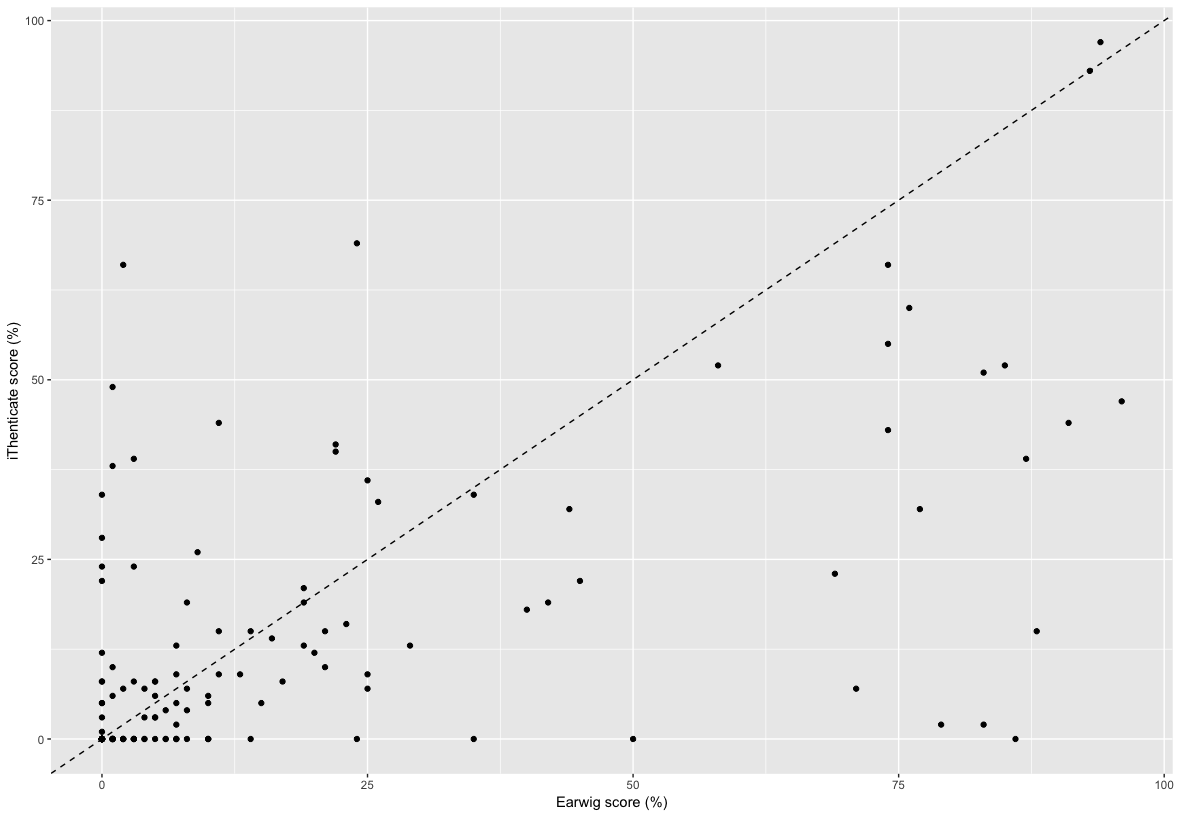
\includegraphics[scale=0.3]{imagenes/1_introduccion}
	\label{1_introduccion}
	\caption{Ejemplo de conjunto de datos \href{https://commons.wikimedia.org/wiki/File:Earwig_ithenticate_scatterplot.png}{(Wikimedia)}}
\end{figure}

Pensemos por ejemplo en este conjunto de datos. Tenemos un cluster muy bien definido en la esquina inferior izquierda y datos dispersos. ¿Podemos afirmar claramente cual es la línea que distingue los datos anómalos de los normales? 

Esta discusión nos lleva a la primera barrera que tenemos que superar en este trabajo. El problema no es resoluble por diseño y por tanto debemos realizar una aproximación a través de los datos. Esto nos va a llevar a aprender de los mismos, valorar cada dato con una puntuación que nos acabará discriminando los datos normales y anómalos.

En el contexto de los problemas resueltos a través de los datos tenemos dos tipos: clasificación y regresión. 

Podríamos pensar que estamos ante un problema de clasificación ordinario, es decir, aprender a través de los datos de entrenamiento cuáles son las anomalías y cuales los datos normales pero no es así. Pensemos que no sabemos ni siquiera nosotros clasificar claramente estas anomalías salvo en algunos ejemplos prácticos. Por ejemplo si le diéramos a una persona un conjunto de datos ya establecido como el que hemos visto anteriormente \ref{1_introduccion} no sería nada fácil e incluso no podemos afirmar que sepamos hacer esta tarea. Por contra si el conjunto de datos es generado en un proceso de trabajo, por ejemplo un conductor de camiones haciendo su ruta, podemos saber cuándo hay una anomalía porque el trabajador la está viviendo y puede señalarla.

Por tanto este problema no es de clasificación al uso pues no es un problema supervisado. Esto significa que, en general no vamos a tener un conjunto etiquetado en el que poder probar cómo aprende nuestro modelo y tendremos que abordar otras técnicas para comprobar el desempeño.

Ahora que comprendemos el alcance del problema podemos intentar profundizar un poco más en la base teórica del mismo analizando las herramientas que el machine learning nos provee para abordarlo.